\chapter{Макросы VBA для проведения расчётов}

Расчёты \unf{} выполняются с использованием макросов, написанных на языке программирования Visual Basic for Application (VBA), встроенном в Excel [\href{https://ru.wikipedia.org/wiki/Visual_Basic_for_Applications}{wikipedia VBA}]. 

Макросы \unf{} могут быть использованы различными способами. В самом простом варианте для использования \unf{} не требуется программировать (писать код на VBA), достаточно уметь вызывать необходимые функции из рабочей книги Excel, создавая расчётные модули. В более сложном и мощном варианте использования на основе функций \unf{} можно создавать свои макросы, которые могут быть вызваны, например, по нажатию кнопки. Это упрощает проведение больших массовых расчётов, но требует написания кода на VBA. Самый продвинутый вариант подразумевает создание собственных программ на основе объектной модели \unf{}. 


Исходный код расчётных модулей находится в отдельном файле - надстройке Excel - файле с расширением.xlam. Для использования макросов данная надстройка должна быть запущена в программе Excel при проведении расчётов. Ее можно каждый раз запускать вручную или установить для автоматического запуска при старте Excel. Подробное описание процедуры установки надстройки можно найти на сайте Microsoft по ключевым словам  \href{https://support.office.com/ru-ru/article/%D0%94%D0%BE%D0%B1%D0%B0%D0%B2%D0%BB%D0%B5%D0%BD%D0%B8%D0%B5-%D0%B8-%D1%83%D0%B4%D0%B0%D0%BB%D0%B5%D0%BD%D0%B8%D0%B5-%D0%BD%D0%B0%D0%B4%D1%81%D1%82%D1%80%D0%BE%D0%B5%D0%BA-%D0%B2-excel-0af570c4-5cf3-4fa9-9b88-403625a0b460}{"добавление и удаление надстроек в Excel"}.


\section{Работа с VBA}



\section{Ручной запуск надстройки}
Для работы с надстройкой рекомендуется ручной способ ее запуска, описанный в данном разделе. (альтернативный способ описан в следующем разделе).
Ручной запуск надстройки не требует ее установки на компьютере. Это бывает удобно, когда версия настройки часто меняется. Для этого необходимо открыть файл надстройки непосредственно в Excel, например двойным щелчком по файлу с расширением.xlam в проводнике. При этом Excel откроется, но никаких документов в нем не появится, а сама надстройка будет загружена и готова к использованию. Надстройка alglib.xlam должна находится в одной папке с надстройкой \unf. Она будет автоматически загружена.
Убедиться, что надстройка загружена можно по наличию закладке "unifloc" на панели кнопок Excel. Там же можно найти кнопку для проверки версии надстройки и исправления путей к надстройке. 

При переносе файла использующего макросы \unf{} на другой компьютер, при запуске может возникать сообщение, что связанный файл надстройки не найден. Это происходит поскольку Excel при использовании функций любой надстройки автоматически при вызове функции сохраняет полный путь к надстройке. При изменении положения надстройки на компьютере (например при переносе на новый компьютер) excel не может автоматически исправить путь и требует действий пользователя.

При получении такого сообщения возможны два варианта действий. Первый - в окне запроса следует выбрать кнопку "изменить"\ и указать правильное положение файла надстройки. Второй - в окне запроса указать - продолжить (или отменить обновление связанных файлов). После того как окно закроется, на закладке "unifloc" выбрать кнопку <<исправить ссылки на надстройку>>. После этого для всех вызовов функций надстройки \unf{} ссылки на надстройку будут исправлены автоматически. Отчёт об исправлении можно найти в окне immediate редактора VBE. 


\section{Установка надстройки для автоматического запуска}
\begin{enumerate}
	\item На вкладке Файл выберите команду Параметры, а затем — категорию Надстройки.
	\item В поле Управление выберите пункт Надстройки Excel, а затем нажмите кнопку Перейти. Откроется диалоговое окно Надстройки.
	\item Чтобы установить и активировать надстройку \unf, нажмите кнопку Обзор (в диалоговом окне Надстройки), выберите файл надстройки, а затем нажмите кнопку ОК.
	\item Аналогично надстройке \unf{} потребуется установить надстройку alglib.xlam 
	\item Надстройка появится в списке надстроек. Галочка активации надстройки должна быть установлена
\end{enumerate}	

После установки и активации надстройки, встроенными в нее макросами можно будет пользоваться в любой книге Excel на данном компьютере. При переносе расчётных файлов на другой компьютер для сохранения их работоспособности должна быть передана и установлена и надстройка. 
При переносе файлов использующих функции \unf{} с другого компьютера или на другой компьютер может потребоваться исправить путь к надстройке. Это можно сделать с использованием соответствующей кнопки на закладке "unifloc".

\section{Редактор VBE}
Чтобы получить доступ к макросам в текущей версии расчётного модуля для выполнения упражнений необходимо:
\begin{itemize}
	\item Запустить Excel запустив рабочую книгу для выполнения упражнений
	\item Нажать комбинацию клавиш <Alt-F11>
	\item Откроется новое окно c редактором макросов VBA (Рис. \ref{ris:VBA_overview}). Иногда в литературе окно редактирования макросов обозначают как VBE (Visual Basic Enviroment)
	\item Окне VBE можно изучить структуру проекта (набора макросов и других элементов). Раздел со структурой проекта можно открыть из меню <Вид – Обозреватель проекта>. Макросы располагаются в ветках «модули» и «модули классов»
	 
\end{itemize}

\begin{figure}[ht]
	\center{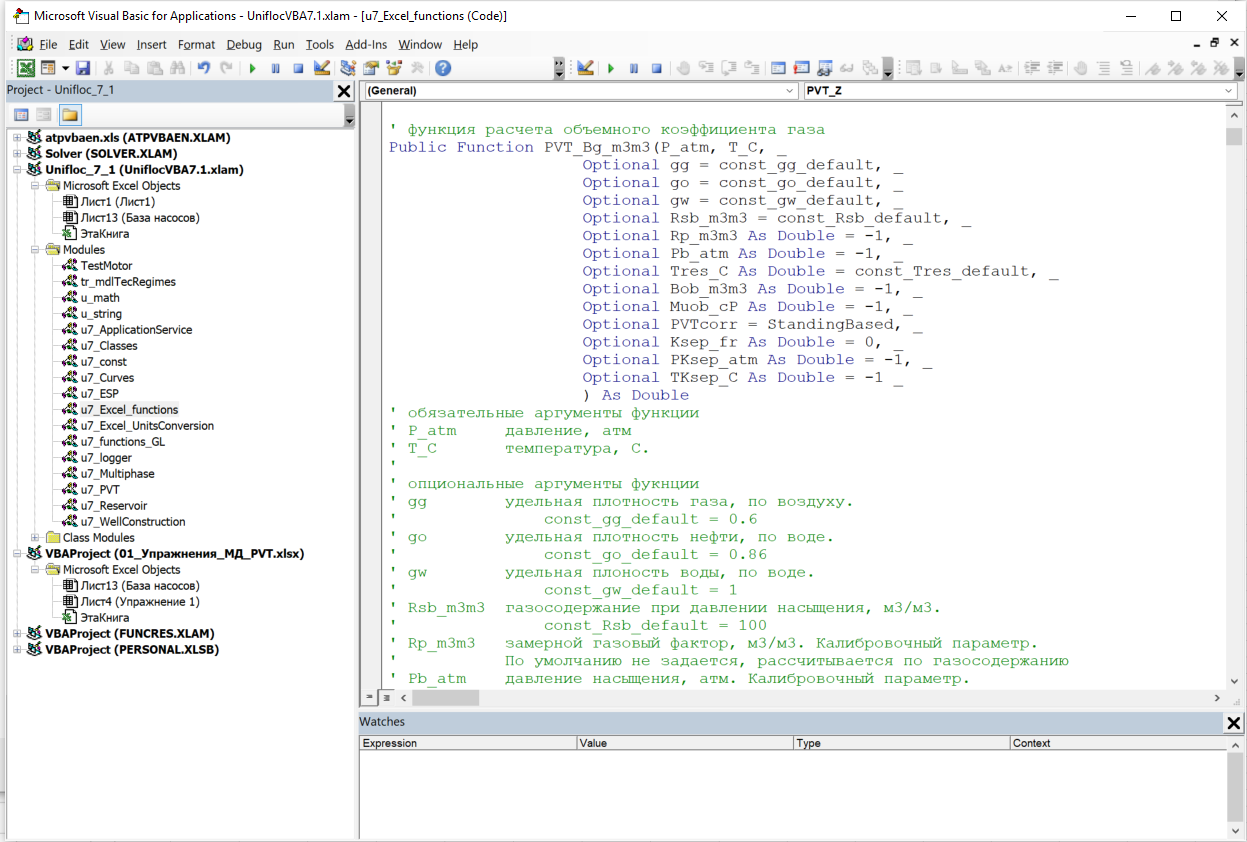
\includegraphics[width=1\linewidth]{vba_overview}}
	\caption{Окно редактора VBE}
	\label{ris:VBA_overview}
\end{figure}


\section{Особенности VBA и соглашения \unf{}}
Строки, начинающиеся со знака ‘ являются комментариями. В VBE они выделяются зелёным цветом. На исполнение макросов не влияют.

Для многих макросов не обязательно задавать все параметры. Некоторые значения параметров могут не задаваться – тогда будут использованы значения параметров, принятые по умолчанию. Параметры, допускающие задание по умолчанию, помечены в исходном коде ключевым словом \mintinline{vb.net}{Optional}.

При создании макросов в основном использовались международные обозначения переменных, принятые в монографиях общества инженеров нефтяников SPE. Список наиболее употребляемых обозначений приведён в приложении. 

При создании макросов для обозначения переменных разработчики старались придерживаться следующих соглашений (не всегда успешно впрочем)
\begin{itemize}
	\item название переменной или функции отражает физический смысл 
	\item лучше длинное и понятное название, чем короткое и непонятное, разделители слов в названиях - знаки подчёркивания (там, где это возможно)
	\item для расчётных функций название может содержать (последовательно) - префикс, указывающий группу функций, расчётное значение, ключевые параметры, на основе которых проводится расчёт, размерность результата
	\item для минимизации путаницы с размерностями физических величин все размерные переменные в названии содержат явное указание размерности
\end{itemize}

